\entry{Semana del 18/08/2025.} 
\section{Lunes 18/08/2025.} 

\subsection*{Posibles nuevos equipos.} 
Pablo estuvo buscando alternativas de generador de funciones y osciloscopio para volver el setup un poco más permanente. Encontró la marca UNI-T con distribuidora oficial en Argentina que posee instrumentos de \textit{aparentemente} muy buena relación calidad precio y de tamaño portátil. 

Los que nos interesarían principalmente son: 
\begin{itemize}
	\item Generador de funciones UTG932e (30 MHz). 
	\item Osciloscopio UTD2052CL. 
\end{itemize}

Ambos están en el rango de precios de aproximadamente \$ 350.000, y en la página de UNI-T cuentan con los manuales e información sobre su manejo vía API, pudiéndose usar con pyvisa. En particular para el generador encontré el siguiente wrapper de la comunidad: \url{https://github.com/jarjuk/UTG900}.    

Otra alternativa es la marca Rigol que cuenta con osciloscopios con generadores de funciones embebidos. \href{https://www.rigolna.com/products/digital-oscilloscopes/1000z/?srsltid=AfmBOooyiYs5EehPOwh3nspDsWKO8ZRaz3G0OwuuPlwIOZEdBgH4wbH2}{Opciones.} Probablemente el más económico/barato en esta línea sea el Rigol DS1074Z-S Plus, pero no sé si hay algún distribuidor en Argentina que lo esté vendiendo, y el precio parece superar el \$ 1.000.000.  

\section{Viernes 22/08/2025.} 

\subsection*{Notas del día:}
\begin{itemize} 
	\setlength\itemsep{0.1em}
	\item Hoy querría empezar a medir en la cuba chica. Idealmente medir para forzados de varias amplitudes crecientes y forzando hasta 4 o 6 Hz y comparar los resultados. Además me gustaría hacer alguna medición con FCD para obtener la relación de dispersión y mostrar cómo a medida que aumenta la potencia inyectada se va ensanchando la relación de dispersión. 
	\item  Generar nuevos forzados con más amplitud cambia la forma de la curva en sí además, no sé si usar entonces esas o simplemente escalar la primera que use. 
	
	\item  Si apago y prendo el generador también aparece la subida/bajada exponencial, pero solo midiendo sobre la resistencia del RLC.  
	
	\item  Ya tengo todo armado, quedó el tornillo micrométrico en 38. Agua a 5.2 cm de altura medido con la reglita metálica.  
	\item  Voy a estar trabajando con 10 Vpp. Frecuencia de resonancia alrededor de 51.983 kHz. 
	\item  La mápxima del motor son un poco menos de 16384 puntos. Voy a trabajar siempre con 16000. 
	\item  Parece que ya está todo funcionando, el factor 1, que va entre -1 y 1 cm va a ser la máxima amplitud y voy a ir bajando. 
	\item  Sobresale por arriba 4.65 cm el fierrito de la paleta, hasta donde se empieza a doblar. 
	\item  Por si fuese relevante la curva se está vaciando. 
	
	\item  Pendiente: Forzar con senos e ir subiendo la amplitud para ver cómo se transforma al régimen turbulento y aparecen otros armónicos a parte de los de la caja. 
	
	\item  Para factor 1 puse recién a medir durante 10 minutos el estacionario, tendría que medir también el ruido, y transitorio al inicio y al final. Lo paré a los 5 minutos. 
	\item  Al prender el motor tener en cuenta que pega el salto hasta la posición inicial, a corregir después. Además buffer overrun. 
	\item Ya solucioné lo del salto, es que estaba puesto el scaling en 50 \%, entonces la posición inicial iba a ser -8.556/2. Para TODAS las mediciones que tomé antes de hoy con el motor asumir que estaba pasando esto. Y además del osciloscopio el error es de $\pm$0.15 mm aprox, y el escalonado era de 0.5/2 mm así que es compatible con eso. 
	\item Voy a ir bajando la amplitud de a 5 \%. Con 50 \% y el salto arreglado vuelvo a medir el transitorio inicial. Cayó la paleta y está tocando el fondo en prender3. 
	\item Prender4 ya debería estar bien.   
	
	\item Voy a tomar siempre 5 minutos. Medí hasta ahora: 50 \%, 45 \%, 40 \%, 35 \%, 30 \%, 25 \%, 20 \% (HASTA ACÁ 51.896 kHz)
	\item Para el de 35 \% sincronicé el osciloscopio con la medida. 
	\item Para 20 \% voy a hacer el prender sin el salto. 
	
	\item Hago para 50 \% con 0-5, 0-6 Hz y para la inversa de 17 a 19 Hz. 
	\item Golpe Durante la de 0-6 Hz. 
	\item Durante la inversa salpica algo de agua. Era de nuevo para 0-6 Hz eso, ahora cargo la inversa. Vibrava demasiado. Lo dejé solo un par de segundos. 
	
	\item Cosas pendientes para el Lunes: Medir con un seno de varias amplitudes, medir con FCD el forzado con amplitudesa crecientes y calcular la relación de dispersión en cada caso. 
	\item Ir viendo cuándo la fase se vuelve realmente aleatoria al aumentar la amplitud del forzado. 
	
	\item Mandar a imprimir otra carcasa para tener otro sensor y empezar a ver funciones de correlación a dos puntos. 
\end{itemize}

\subsection*{Turbulencia de Ondas en la Cuba Chica.} 
Empecé a realizar experiencias típicas de WT en la cuba chica. Para eso usé el Setup que está descripto más abajo. 

\begin{figure}[th!]
	\centering
	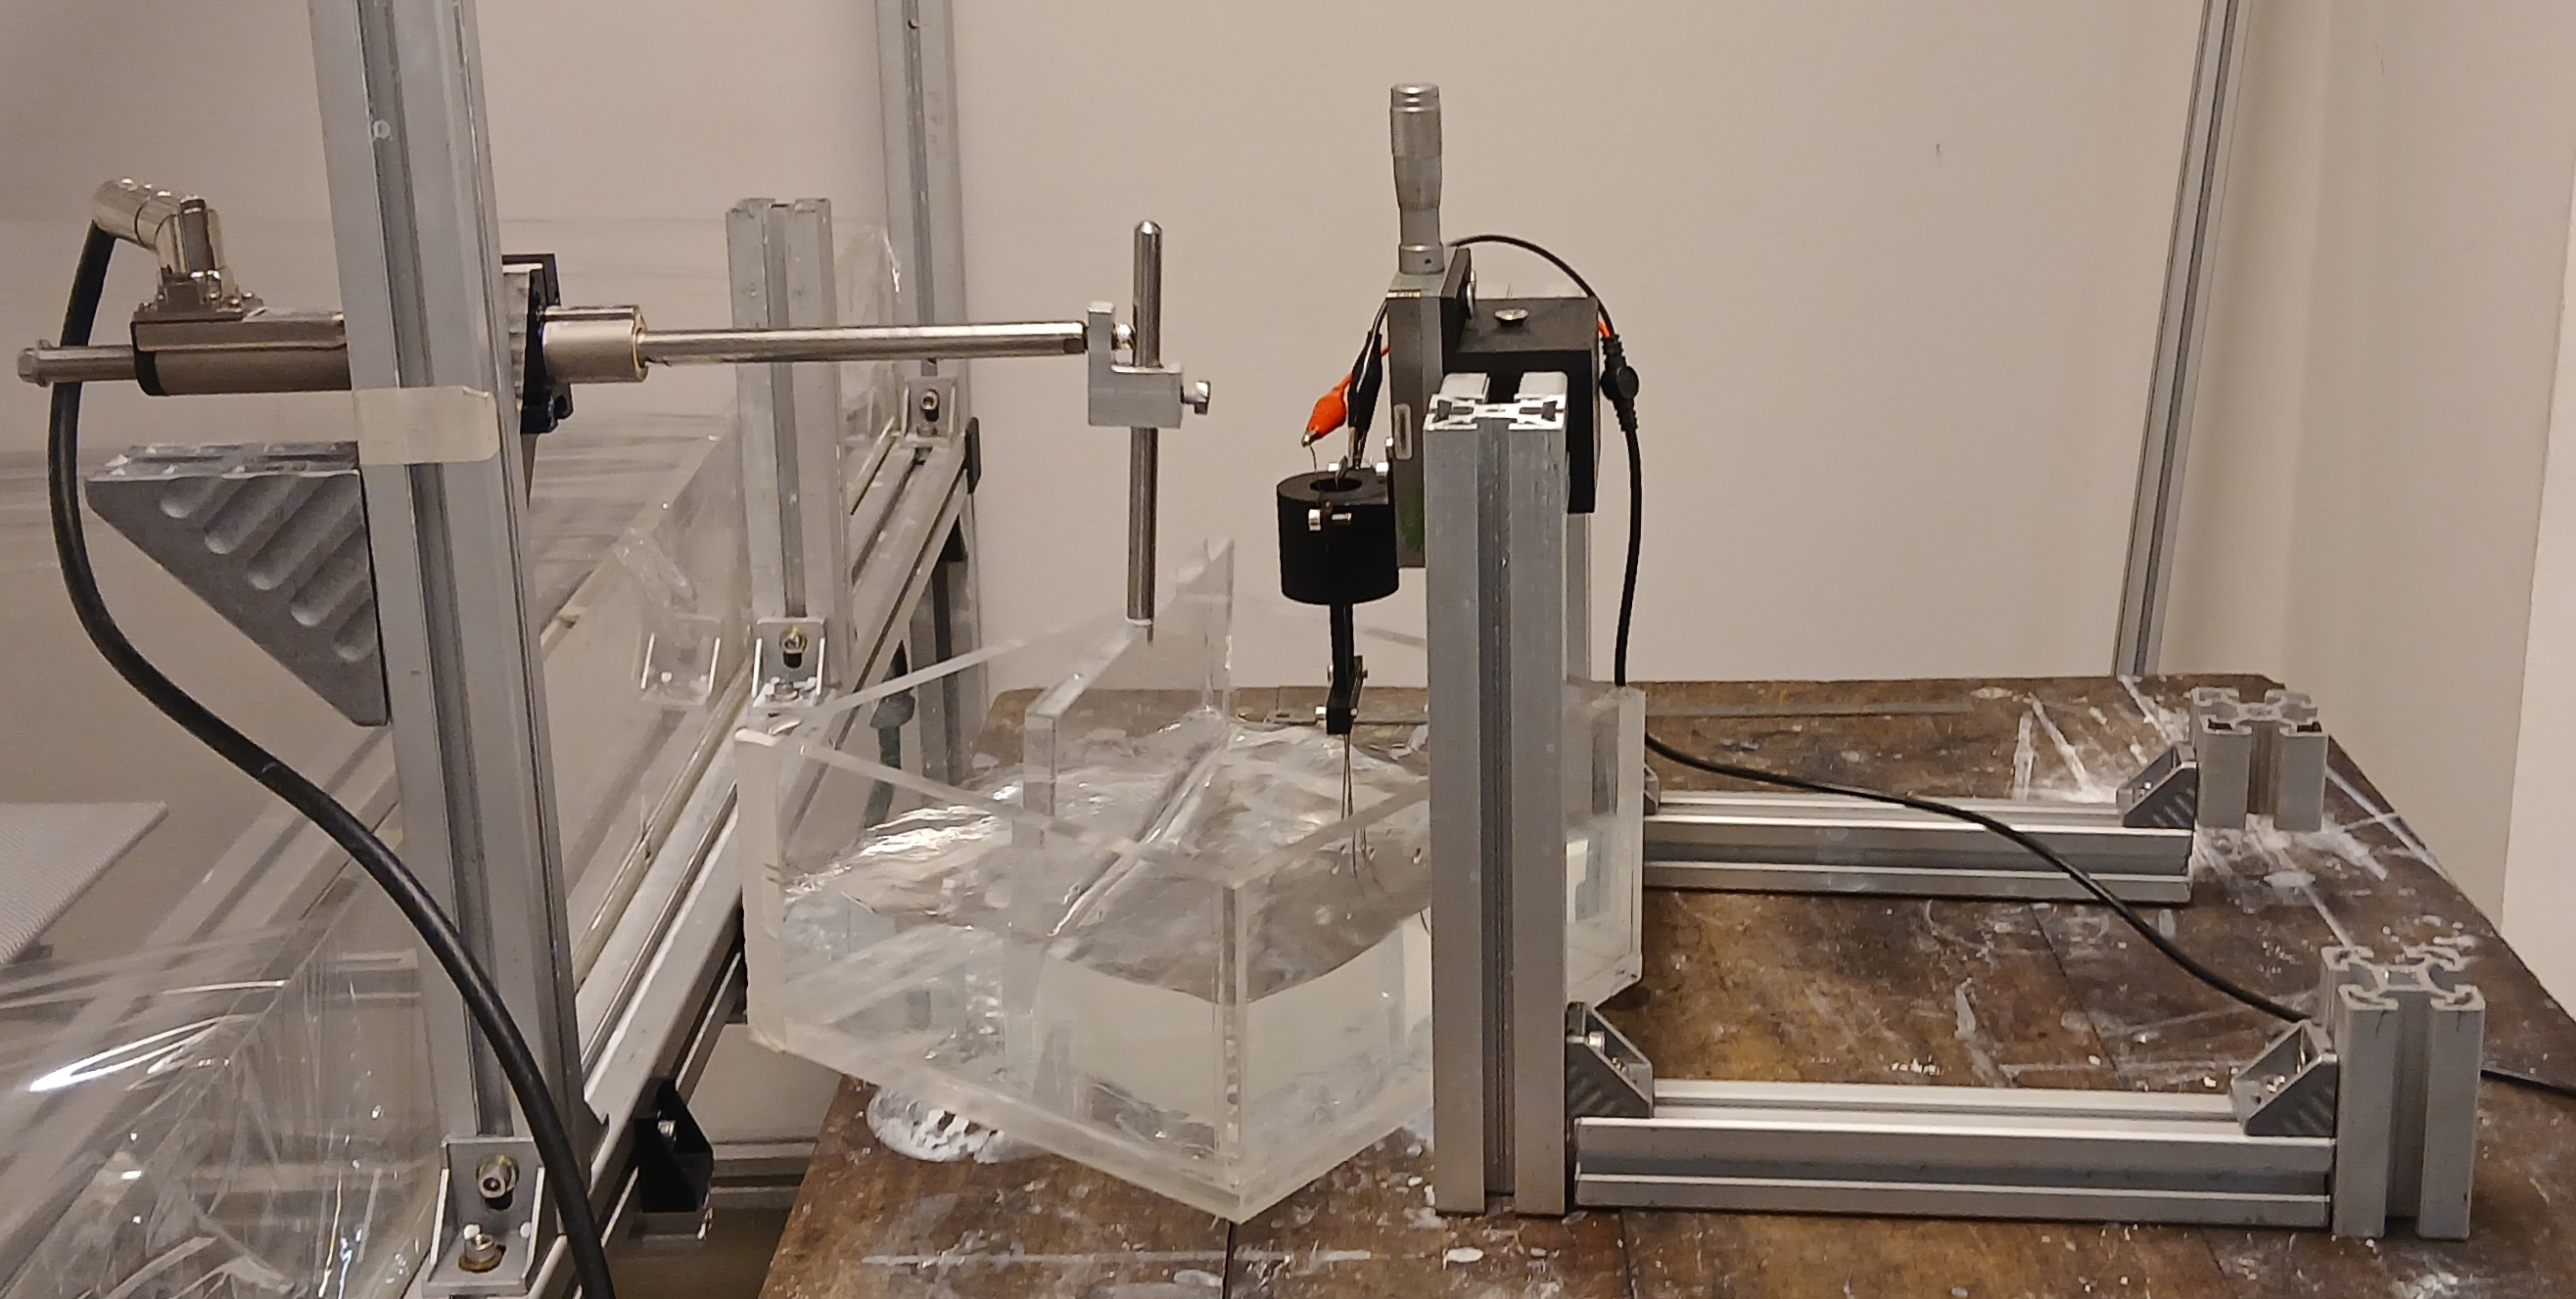
\includegraphics[width=0.897\linewidth]{Figures/18_08_2025/Setup_cuba_chica_sensor}
	\caption{Setup para estudiar en la cuba chica la respuesta del fluido a un forzado aleatorio en una banda de frecuencias de entre 0 Hz y hasta 4-6 Hz y varias amplitudes, mediante un solo wave-driver puesto un poco en diagonal. Acá estoy midiendo puntualmente la altura local de la superficie libre con el sensor capacitivo.}
	\label{fig:setupcubachicasensor}
\end{figure}


